\section{Deriving a log repair}
\label{sec:sol}
In this section, we 
introduce a basic solver-based approach to 
resolve the incorrectness reflected by the complaints. 
This approach 
constructs a mixed-integer linear 
programming (MILP) problem by
linearizing and parameterizing the 
original query log over tuples
in the database. 
\subsection{Linearizing \& Parameterizing Single Query}
\label{sec:linearize}
% describe how to linearize a single query
We linearize and parameterize a query $q$ by considering its effects on the 
targeted table $R(A_1, ..., A_m)$: we treat the query $q$ as a 
conditional function over each tuple $t\in R$ and convert the effects of $q$ 
over $t$ into a set of linear inequality constraints. 
\subsubsection{Query as a Conditional Function}
The effect of query $q$ over a tuple $t$ can be expressed in a conditional
function $f_q(t)$ as the following:
\begin{definition} [Conditional Function]
\label{def:cond}
	The conditional function for query $q$ is:
	\[
    f_q(t)= 
\begin{cases}
    f_{q.\mu} (t) ,& \text{if } f_{q.\sigma} (t)\\
    t,              & \text{otherwise}
\end{cases}
\]
$f_{q.\mu}$ is the \textit{update function} consists of
 a set of \textit{update equation(s)};\\
 $f_{q.\sigma}$ is the 
 \textit{condition function} consists of a 
set of \textit{logical expression(s)} in 
disjunctive or conjunctive form.
\end{definition} 

 This conditional function applies 
to all kinds of \emph{update queries} (Section~\ref{sec:model}): \\
\texttt{UPDATE} query: $f_{q.\mu}(t)$, $f_{q.\sigma}(t)$ reflects the 
equations in
set clause and the expressions in where clause over attributes in
$R$. \\
\texttt{INSERT} query: $f_{q.\mu}(t)$ reflects the inserted values in
values clause and 
$f_{q.\sigma}(t)$ is a boolean variable 
reflects the existence of tuple $t$; 
$\vee_{t\in R} f_{q.\sigma}(t)$ 
represents
the existence of this insert query.  \\
\texttt{DELETE} query: $f_{q.\mu}(t)$ reflects the deleted values for 
each attribute and 
$f_{q.\sigma}(t)$ reflects the expressions in where clause (similar to
$f_{q.\sigma}(t)$ in \texttt{UPDATE} query).

\smallskip

We parameterize query $q$ by replacing 
 all numeric values 
in the above conditional function into
undetermined variables (Example~\ref{ex:parameterize}).
\begin{example}\label{ex:parameterize}
Consider a \texttt{UPDATE} query $q$:
\texttt{UPDATE R SET A$_1$ = 3 WHERE A$_2$ $\leq$ 10},
the conditional function of this query is: 
\[
    f_q(t)= 
\begin{cases}
    f_{q.\mu}(t) = \{t.A_1 = 3\} ,& \text{if } f_{q.\sigma}(t) = \wedge\{t.A_2 \leq 10\}\\
    t,              & \text{otherwise}
\end{cases}
\]
The numeric variables in query $q$ including \texttt{3} in $f_{q.\mu}(t)$ and \texttt{10}
in $f_{q.\sigma}(t)$. Thus, we parameterize query $q$ by replacing the value \texttt{3, 10}
by two undetermined variables \texttt{var1, var2}. 
\end{example} 
\subsubsection{Constructing Linear Inequality Constraints}
We linearize query $q$ by transforming its conditional function 
over each tuple $t\in R$ into a set of linear (in)equality constraints. \\
According to Definition~\ref{def:cond}, 
the updated value $t'$ for tuple $t$ in attribute $A_i$ can be expressed as  
\begin{eqnarray}
\label{eq:linearization}
t.A_i' = x\otimes f_{q.\mu(A_i)} (t.A_i) + (1-x)\otimes t.A_i. 
\end{eqnarray} 
Linearizing Equation~\ref{eq:linearization} is equivalent as linearzing
query $q$.  
To linearize Equation~\ref{eq:linearization}, 
we first introduce a boolean variable $x$ to represent the satisfactory 
of tuple $t$ on the condition function of query $q$:
\begin{eqnarray}
\label{eq:x}
x = f_{q.\sigma}(t)
\end{eqnarray}

We then create two set of intermediate variables,
$u=\{u.A_1, ..., u.A_m\}$, $v = \{v.A_1, ..., v.A_m\}$, 
for each attribute $A_i$ in tuple $t$:
\begin{eqnarray}
\label{eq:uv}
u.A_i &\leq & f_{q.\mu(A_i)} (t.A_i) \nonumber\\
u.A_i &\leq & xM \nonumber\\ 
u.A_i &\geq & f_{q.\mu(A_i)} (t.A_i) - (1-x)M ; \nonumber \\\nonumber \\
v.A_i &\leq & t.A_i \nonumber\\
v.A_i &\leq & (1-x)M \nonumber\\
v.A_i &\geq & t.A_i - xM
\end{eqnarray}
Here, $M$ denotes a very large number (greater than the upper bound for the $t.A_i$).
By doing so, we may express Equation~\ref{eq:linearization} as:
\begin{eqnarray}
\label{eq:tnew}
t.A_i' = u.A_i + v.A_i
\end{eqnarray}
By combining these linear (in)equality constraints 
(~\ref{eq:x}~\ref{eq:uv}~\ref{eq:tnew}), we form the transformation 
of a single attribute $A_i$ from a single tuple $t$ 
by a single query $q$. To fully linearize a query, 
similar constraints should be
derived for the other attributes and the other tuples. 

\subsection{A Basic Solver-based Approach}
\label{sec:milp}
Using the linearization
 method in Section~\ref{sec:linearize}, we can further
linearize
the entire query log by converting every tuples in the table $R$. 
During the linearization, we further parameterize each
query in the query log $\mathcal{Q}$ in order by 
derive the log repair. 
The linearized and parameterized query log
should start from and end at clean database states.
To achieve this, we add constraints
by assigning the true initial and end database 
states' values (based on complaints) 
to the corresponding variables. 
Following the above steps 
(Algorithm~\ref{alg:basic}), we convert the 
query log into a collection of constraints 
with newly introduced variables. 
Some of these variables
are introduced to linearize the query log 
and the rest usually
represent the numeric values in the query log
during the paramerization process. 
The latter set of 
variables often involved in the objective function 
according to the pre-defined distance function $d$ 
(as described in Definition~\ref{def:problem}). \\

\begin{algorithm}[htbp]
\caption{A Basic Solver-based Approach}
\label{alg:basic}
\begin{algorithmic}
\REQUIRE {$\mathcal{Q}, D_0, D_n, \mathcal{C}$}
\ENSURE {$\mathcal{Q^*}$}
\STATE $milp\_cons \leftarrow \emptyset$
\FOR {each $t$ in $R$}
\FOR {each $q$ in $\mathcal{Q}$}
\STATE $milp\_cons \leftarrow milp\_cons \cup LinearAndParam(q, t)$
\ENDFOR
\STATE $milp\_cons \leftarrow milp\_cons \cup AssignVals(D_0.t, D_n.t, \mathcal{C})$
\ENDFOR 
\STATE $milp\_obj \leftarrow FormObj (milp\_cons, \mathcal{Q})$
\STATE $solved\_vals \leftarrow MILPSolver(milp\_cons, milp\_obj)$
\STATE $\mathcal{Q}^* \leftarrow ConvertQLog(Q, solved\_vals)$
\STATE Return $\mathcal{Q}^*$
\end{algorithmic}
\end{algorithm}
By constructing linear (in)equality constraints and
defining a objective function, we convert the problem into
 a mixed-integer linear programming (MILP) problem that can be 
 solved by MILP solvers. By solving this MILP problem, we collect the
corrections for the parameterized variables and form the log repair. 
% describe how to linearize the whole querylog with provided
% database states info. 
\section{Optimizing the Basic Approach}
\label{sec:opt}
In the previous section, we introduce the basic approach to derive
the log repair by incorporating information from every query
and every tuple into a single MILP problem. However, oftentimes, 
this basic approach end up with 
a huge problem as the query log size and table size increase. 
In Figure~\ref{fig:querysize_vs_time}, 
\begin{wrapfigure}{R}{0.25\textwidth}
    \centering
        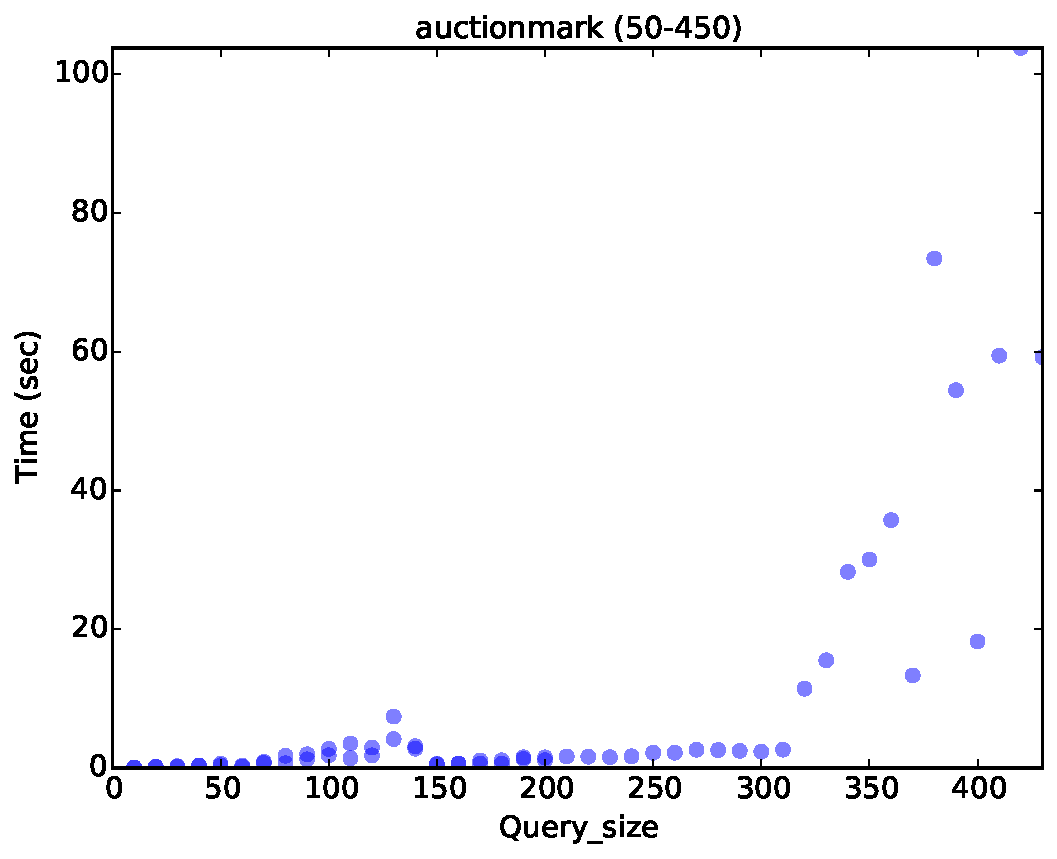
\includegraphics[width=0.25\textwidth]{figures/auctionmark_qsize_time}
    \caption{\# of queries vs. execution time on Auctionmark dataset. }
    \label{fig:querysize_vs_time}
\end{wrapfigure}
we observe that the total solver (IBM CPLEX) solving time 
grows exponentially and 
unpredictably as the query 
log size increases. As a result, the basic approach does not scale over 
large problems (large query log size and large table size).\\
To resolve the scalability limitation of the basic approach, 
we try to optimize
the basic approach in multiple different ways:

\smallskip

\noindent \textbf{Chunk query log \& Rollback (failed):} \\
A natural idea to optimize the basic approach is 
to \textbf{chunk the query log} into
smaller, fixed size pieces and then solve each piece at a time: starting
from the most recent piece, the system linearizes and parameterizes queries 
in the current piece and derives a corresponding log repair; 
it then examines the other pieces iteratively
in the same way. Since complaints only provides
true values for the most recent database state, in order to avoid 
linearizing additional queries, 
we need to know \textbf{rollback} the true values of tuples 
until the last query in each query log piece. \\
However, rollback the database is non-easy. An ideal, precise rollback
algorithm would generate a set of valid ranges for each attribute of a tuple. 
But the size of valid ranges also grows exponentially with the number queries
we want to rollback, which, in turn, could not improve the system performance. 
On the other hand, an approximate, imprecise 
rollback algorithm would either make the rest of the problems
infeasible to solve (only maintain fixed number of valid ranges) 
or result in deriving 
incorrect log repairs (maintain the lower 
bound and upper bound among all valid ranges).
  
\smallskip

In order to improve the system performance without losing accuracy, we propose
the following two optimizations: query-slicing optimization 
based on provenance over queries and
attribute-slicing optimization based on provenance over 
attributes. 
\subsection{Query-slicing Optimization}
\label{sec:opt:query}
Parameterizing the full query log as in the basic approach 
is often unnecessary as many queries in the query log 
are indeed irrelevant to the complaints.
To avoid such redundant computation, we use the \textit{query-slicing} 
ptimization to prune out irrelevant queries. The \textit{query-slicing} 
optimization first searches for all attributes that may modified by a query, 
it then compares these attributes with the actual incorrect ones (according
to the complaints), and finally decides whether this query is relevant or not.
\begin{definition} [Incorrect Attributes]
	The incorrect attributes $\mathcal{A}(C)$ are attributes in 
	table $R$ with incorrect values: 
	\[\mathcal{A}(C) = \{A_i|A_i\in R, \exists t.A_i \neq t.A_i^*, t\in C\}\]
\end{definition} 
\begin{definition}[Query dependency\& impact]
    The \textbf{dependency}, $\mathcal{P}(q)$, of a query $q$
    is the set of 
    attributes involved in the condition function of $q$:
    \[\mathcal{P}(q) = \Pi_{f_{q}.\sigma}(R)\]
    The \textbf{direct-impact} of query $q$, denoted
    by $\mathcal{I}(q)$, is the set of attributes 
    involved in the update function of $q$:
    \[\mathcal{I}(q) = \Pi_{f_{q}.\mu}(R)\]
    The \textbf{full-impact}
    of $q$, $\mathcal{F}(q)$, includes all attributes 
    that may modified by $q$.  
\end{definition}
By comparing $\mathcal{F}(q)$ and $\mathcal{A}(C)$, we know whether
query $q$ can solve the problem or not: when $|\mathcal{F}(q) \cap 
\mathcal{A}(C)|=|\mathcal{A}(C)|$, query $q$ may solve all incorrect 
attributes; when $0 < |\mathcal{F}(q) \cap 
\mathcal{A}(C)|< |\mathcal{A}(C)|$, query $q$ may solve part of the 
incorrect attributes; and when $|\mathcal{F}(q) \cap 
\mathcal{A}(C)|=0$, query $q$ is irrelevant and should not be 
parameterized. We use $Rel\mathcal{(Q)}$ 
denotes the set of relevant queries. 
Algorithm~\ref{alg:fullimpact} describes how we find
$\mathcal{F}(q)$ for all queries in the query log.
\begin{algorithm}[htbp]
\caption{Find Full-impact}
\label{alg:fullimpact}
\begin{algorithmic}
\REQUIRE {$\mathcal{Q}$}
\ENSURE {$\mathcal{F}(\mathcal{Q})=\{\mathcal{F}(q_1), ..., \mathcal{F}(q_n)\}$}
\FOR {each $q_i$ in $q_n, ..., q_1$}
\STATE $\mathcal{F}(q_i) \leftarrow \mathcal{I}(q_i)$
\FOR {each $q_j$ in $q_{i+1}, ..., q_{n}$}
\IF {$\mathcal{I}(q_i)\cap \mathcal{P}(q_i) \neq \emptyset$}
\STATE $\mathcal{F}(q_i) \leftarrow \mathcal{F}(q_i) \cup \mathcal{F}(q_j)$
\ENDIF
\ENDFOR
\STATE $\mathcal{F}(\mathcal{Q}) \leftarrow \mathcal{F}(\mathcal{Q}) \cup \mathcal{F}(q_i)$
\ENDFOR
\STATE Return $\mathcal{F}(\mathcal{Q})$
\end{algorithmic}
\end{algorithm}
\subsubsection{Attribute-slicing Optimization}
In addition to pruning out irrelevant queries,
we also prune irrelevant attributes. \\
Let $Rel\mathcal{(Q)}$ as the set of 
relevant queries, we can find the relevant 
attributes as following:
\[Rel\mathcal{(A)} = \cup_{q_i \in Rel\mathcal{Q)}} 
(\mathcal{F}(q_i)\cup \mathcal{P}(q_i)) \]
\subsection{Attribute-slicing Heuristic}
\label{sec:heurstic}
To further improve efficiency, we propose the attribute-slicing heuristic 
(Algorithm~\ref{alg:heu}) that may lose accuracy. This attribute-slicing
heuristic iteratively
generates the log repair by splitting the relevant 
attributes $Rel\mathcal{(A)}$ into
groups and fixing parameters involved 
in each group separately through a 
much smaller MILP problem. By 
controlling the number of attributes 
in each group, we bound the size of 
each MILP problem in the repair process.
\begin{algorithm}[htbp]
\caption{Attribute-slicing Heuristic}
\label{alg:heu}
\begin{algorithmic}
\REQUIRE {$\mathcal{Q}, D_0, D_n, \mathcal{C}$}
\ENSURE {$\mathcal{Q^*}$}
\STATE $Rel\mathcal{(A)} \leftarrow FindRelAttr(\mathcal{Q}, D_n, \mathcal{C})$
\STATE $Rel\mathcal{(Q)} \leftarrow FindRelQuery(\mathcal{Q}, D_n, \mathcal{C})$
\STATE $\mathcal{G} \leftarrow SplitAttr(Rel\mathcal{(A)})$
\STATE $solved\_vals \leftarrow \emptyset$
\FOR {each $\partial (Rel\mathcal{(A)})$ in $\mathcal{G}$}
\STATE $\mathcal{Q'} \leftarrow PartialCF(\mathcal{Q}, \partial (Rel\mathcal{(A)}))$
\STATE $solved\_vals \leftarrow BasicApproach(\mathcal{Q'}, solved\_vals, ...)$
\ENDFOR
\STATE $\mathcal{Q}^* \leftarrow ConvertQLog(Q, solved\_vals)$
\STATE Return $\mathcal{Q}^*$
\end{algorithmic}
\end{algorithm}

In order to construct the sub MILP problem 
for a attribute group, we rewrite the conditional 
function, $f_q(t)$, into 
the partial conditional function format, $\partial (f_q(t))$.

\begin{definition} [Partial Conditional Function]
	The partial conditional function for a query $q$ over 
	attribute set $\partial(Rel\mathcal{(A)})$ is:
	\[
    \partial (f_q(t))= 
\begin{cases}
    \partial (f_{q.\mu} (t)) ,& \text{if } \partial (f_{q.\sigma} (t))\\
    t,              & \text{otherwise}
\end{cases}
\]
where
\begin{eqnarray*}
\partial (f_{q.\mu} (t)) &=& \{f|f\in f_{q.\mu}(t), \Pi_{f}(R) 
\in \partial (Rel\mathcal{(A)})\}\\
\partial (f_{q.\sigma} (t)) &=& \cup_{f \in f_{q.\sigma} (t)} \partial(f)
\end{eqnarray*}
Note that $\partial(f)$ is a transformation over a function 
(logical expression) $f$ defined
as following:
\[
\partial(f) = 
\begin{cases}
x,\ if\ \Pi_{f}(R) \cap \partial(Rel\mathcal{(A)}) = \emptyset\\
f, otherwise
\end{cases}
\]
$x$ is a newly introduced boolean variable. 
\end{definition} 
By doing so, we can easily construct the sub MILP problem 
in the same way as in the basic approach. Note that 
after each iteration, the solved variables, 
especially boolean variable $x$(s), are reused to provide 
constraint(s) for attributes that have not been examined. 
We demonstrate the process in Example~\ref{ex:heurstic}.

\begin{example}\label{ex:heurstic}
In this example, we demonstrate how to use Attribute-slicing heuristic to
solve the problem in Example~\ref{ex:taxes}. According to
Section~\ref{sec:opt}, we have:
\begin{eqnarray*}
\mathcal{F}(q_1) &=& \{rate, owed \} \\
\mathcal{F}(q_2) &=& \{owed\} \\
\mathcal{F}(q_3) &=& \{ID, rate, income, owed\}\\
Rel(\mathcal{A}) &=& \{ID, rate, income, owed\}
\end{eqnarray*}
Let us split the relevant attributes into groups: \\ 
$\{\{rate\}, \{owed\}, \{income\}, \{ID\}\}$.\\
Consider the first attribute group $\{rate\}$, we 
first rewrite the query log into $\partial(f_q(t))$ as the following:\\
\begin{minipage}{0.7\textwidth}
    \begin{minipage}[t]{0.2\textwidth}
        \begin{align*}
            f_{q_1.\mu} &=& \{\{rate = 30\}\}; \\
f_{q_2.\mu} &=& \emptyset;  \\
f_{q_3.\mu} &=& \{\{rate = 25\}\};
        \end{align*}
    \end{minipage}
    \hspace{4em}
    \begin{minipage}[t]{0.2\textwidth}
        \begin{align*}
           f_{q_1.\sigma} &=& x_1\\
            f_{q_2.\sigma} &=& true\\
           f_{q_1.\sigma} &=& x_3
        \end{align*}
    \end{minipage}
\end{minipage}

\smallskip

\indent We construct a sub MILP problem by linearizing
this query log over tuple $\{t_1, t_2, t_3, t_4\}$, parameterizing
the numeric variables, $30 and 25$, into $var1, var2$,
and setting the objective function as the minimum Euclidean
distance between modified numeric variable with original ones.
This sub MILP problem provides the following values: $var1 = 30, 
var2 = 25$;$t_1.x_1 = false, t_1.x_3 = false$; $ t_2.x_1 = true, 
t_2.x_3 = false$; $t_3.x_1 = false, t_3.x_3 = false$;
$t_4.x_1 = false; t_4.x_3 = true$.

\smallskip

In next iteration, we focus on attribute group $\{owed\}$ and find
the only numeric variable in $q_2$ should be $100$.
We then examine attribute group $\{income\}$, since we solved
$t_3.x_1 = false$ in the first iteration, the numeric 
variable $85700$ in the where clause of $q_1$ has to be 
changed into $86000+\epsilon$, where $\epsilon$
is a small number less than the minimum gap among values in
attribute $income$. Finally, we check attribute group
$\{ID\}$, and derive a log repair by revise $q_1$ as
\texttt{UPDATE Taxes Set rate = 30 WHERE income >= 86000+$\epsilon$ }. 
\end{example}

\subsection{Handling Noises}
\label{sec:noise}
\subsubsection{False Negatives}
Deal with noise

\subsubsection{False Positives}
Bipartite graph \& density stuff